\documentclass[twoside, a4paper, 12pt]{article}

%Package Settings

\usepackage[utf8]{inputenc}
\usepackage[margin=2.5cm, includefoot]{geometry}
\usepackage{setspace}
\doublespacing
\usepackage[backend=biber,authordate-trad]{biblatex-chicago}
\addbibresource{Refs.bib}
\usepackage{graphicx}
\usepackage{csquotes}
\usepackage{fancyhdr}
\usepackage{titling}
\usepackage[hidelinks]{hyperref}
\usepackage{wrapfig}
\usepackage{float}
\usepackage{caption}
\usepackage{soul}

% Page Style Stuff
\fancypagestyle{plain}{
  \fancyhf{}
  \renewcommand{\headrulewidth}{0.1pt}
  \renewcommand{\footrulewidth}{0.4pt}
  \fancyfoot[LE,RO]{\theauthor}
  \fancyfoot[C]{\thetitle}
  \fancyfoot[RE,LO]{Page \thepage}
}

% Title Formatting
\title{Greek Battle Strategy And Its Victory \\ Over the Achaemenid Empire}

\author{Luke Hedt}
\date{\today}

\setul{}{0.2pt}

% Allows for sourcing images
\newcommand{\sourceL}[1]{\caption*{Source: {#1}\hfill} }
\newcommand{\sourceR}[1]{\caption*{\hfill Source: {#1}} }

% Handy Citation Notes for later:
% \footcite[200]{morris_powell_2010} %To add page numbers to citations
% \blockquote{} % If you plan to quote a huge section of Herodotus

\begin{document}

\pagenumbering{Alph}
\begin{titlepage}
    \centering
    
\includegraphics[width=0.25\textwidth]{UniLogo.png}\par\vspace{1cm}
    {\scshape\Large THE UNIVERSITY OF MELBOURNE \\
              \large ANCW20022 Ancient Greece: \\
              History and Archaeology Essay\par}
    \vspace{1.5cm}
    {\Huge \thetitle \par}
    \vfill

% Bottom of the page
    {\Large\itshape \theauthor \hspace{1em} -- \hspace{1em} 832153 \par}
    \vspace{1.5cm}
    {\Large \today}
\end{titlepage}
% Format first page correctly.
\pagestyle{plain}
\pagenumbering{arabic}

The early fifth century BC was a pivotal period in the formation of the Hellenic
identity, marking the decisive point between the period of \emph{p{\'o}leis} Greece
and the true Hellenic period. The cornerstone of this identity formation
was the defeat of Persia in the Greco-Persian Wars, beginning in 499 BC
with the Ionian Revolt. But what brought about the defeat of Persia? What tactics
were the Greeks employing in the period that brought about their victories?
This essay will attempt to address these questions, discussing how their
strategies and arms and armour were instrumental in the defeat of Persia
in the Greco-Persian Wars.

\par\vspace{1em}

\begin{wrapfigure}{R}{0.4\textwidth}
  \centering
  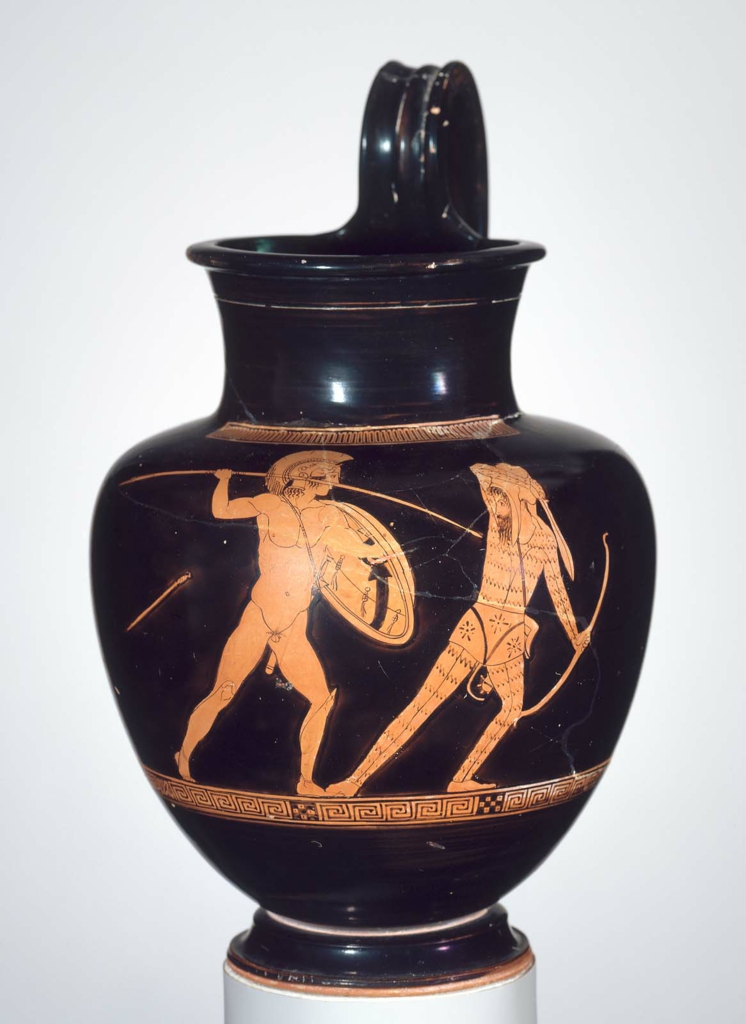
\includegraphics[width=\linewidth]{HopliteArcher.jpg}
  \captionsetup{justification=raggedleft}
  \caption{\ul{ Pottery art of a Greek Hoplite attacking a Persian Archer, circa 450 BC.}}
  \sourceR{\cite{MFABoston_2017_hoplite}}
  \label{img:HopliteArcher}
\end{wrapfigure}

The Greek City States were not a cohesive unit at the outbreak of the fifth century
BC as we tend to think of them today. Rather each urban centre (the
\emph{polis}) controlled
the land around it, and considered itself a separate
However, most of the Greek city states often equipped
themselves rather similarly, copying the armour style of Sparta, the most
effective fighting force in the locality.
The Greek armies are famous for their \emph{hoplite} infantry units, heavily
armoured spear infantry with a distinctive large wooden shield. The shield is
the most important common component, appearing first with the
identifiable double handle in pottery art
circa 700 BC.\footnotemark
The shield was an integral part of infantry kit, being the key defence in battle,
protecting the soldier's front from both the spears and swords of the enemy
infantry, and from arrows from the sky.
Most artistic interpretations of hoplites tend to resemble the pottery
style in \textbf{Figure \ref{img:HopliteArcher}}, spear in the overhand
position and the shield protecting the left-hand side of the body.

\par\vspace{1em}

The widely accepted view is that these depictions are in a `heroic' pose, and not
reflective of real spear techniques. An alternative idea exists
that the technique is actually early hoplite tactics and not just an artistic
pose,\footnotemark[\value{footnote}] however the technique has several issues from
a fighting perspective.
\footnotetext{\cite[57]{wees_hoplite_bronze}}
Firstly, holding the spear in such a way loses one of the main advantages of a
long spear; keeping the enemy at a distance.
To get a balanced spear in the overhand grip, you're required
to keep over half the spear behind your back. Not only do you lose the reach here,
but you're probably going to hit the man behind you in the head because you
can't see what you're doing. It would be far more likely that any weapon held
this way would have a large counterweight on the butt of the spear, keeping it short
and balanced, but the Greeks never used such weapons in art, and none have been found.
Secondly, such a hold is very taxing on the biceps. As strong as Greek men may have been
in antiquity, it seems unlikely that anyone could be bothered holding a spear
up for the duration of a fight when you can use your elbow as a lever in
an under-arm grip.

\par\vspace{1em}

Several schools of thought exist regarding the early hoplite formations. The
main two argue the density of formations, based on where the man held his shield.
Victor Davis Hanson argues that the shield implies a tight formation wherein
a solider must rely on his right-hand neighbour's shield for protection, and
that the shield was an adaptation for a more useful dense formation.\footnotemark
\footnotetext{\cite{hanson_keegan_2009}, found through
    \cite[58]{wees_hoplite_bronze}}
Certainly this is quite a possibility for the well trained Spartans, with a
trust built up over a lifetime of training together. However for the less
professional Ionian armies, it seems less likely that a man would be
willing to trust his life to someone he's barely trained with. Certainly
in the context of the Battle of Marathon, wherein the Athenians
`were sent forth and charged the foreigners at a run,'
\footcite[Book 6.112]{herodotus_1920} Van Wees' argument of the hoplites taking
a more side-on position behind the shield fits much better.
This formation would also require no dependency on your
fellow soldier, \footcite[58]{wees_hoplite_bronze} making it more adaptable to
the one-on-one confrontations pictured in the pottery art.

\par\vspace{1em}

Hoplite armour from here tends to vary a lot more. The hoplites
were usually drawn from the classes that could afford the
equipment, \footcite[38]{wietzel_wheeler_1970}
so each hoplite was probably armoured differently, with gear
missing if it couldn't be purchased. The next main pieces of armour a hoplite
would be wanting were usually their Corinthian helmet (the famous horsehair
ones, though they didn't always have the horsehair) and probably a pair of greaves.
Van Wees argues that due to a limited number of greaves in archaeological finds,
perhaps only a third of hoplites wore them, \footcite[50]{wees_2004} possibly given
that military kit was expensive. Certainly a helmet would have been a priority
over leg armour given how delicate the human head is. Finally, a hoplite would
wear a corselet, bronze body armour held together with leather and bronze banding.
About one in ten hoplites wore the corselet,\footcite{wees_1997} based on
archaeological findings. As the rarest part of the main kit,
it was probably the most expensive, and least necessary given the
hoplite would have a shield to keep enemy weapons out of his torso. Most hoplites
would have also carried a sword, in case his spear broke or for whatever reason
he needed to engage in close combat with an enemy. This was not an uncommon
practice, though it was usually not the primary weapon of choice as the spear
has the advantage of length. \footcite{snodgrass_2006}

\par\vspace{1em}

\begin{wrapfigure}{L}{0.4\textwidth}
  \centering
  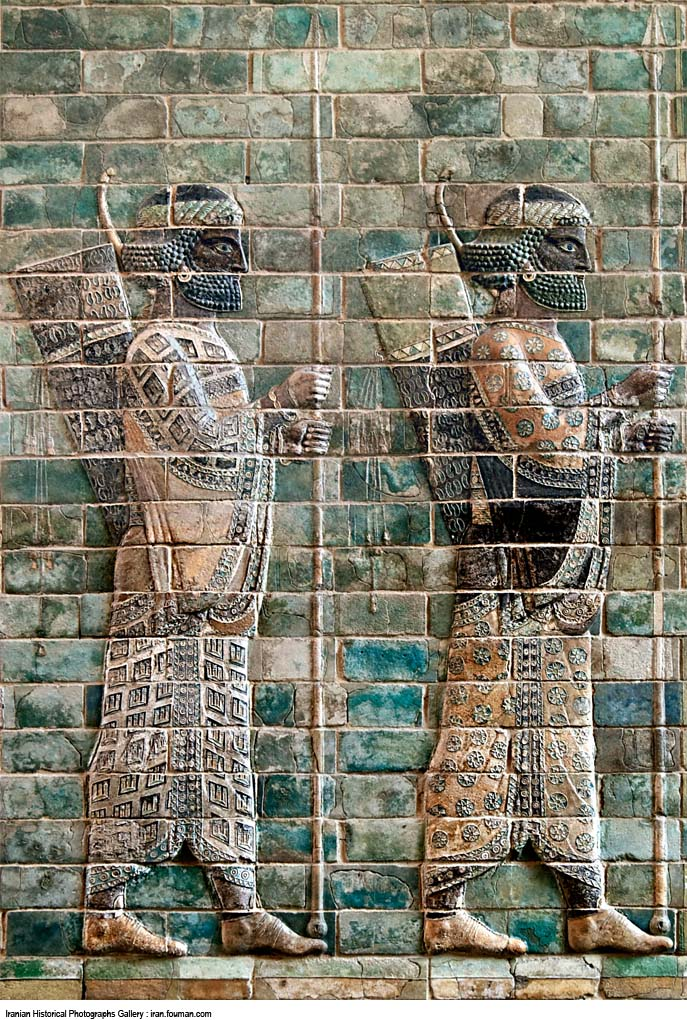
\includegraphics[width=\linewidth]{ImmortalsSusa.jpg}
  \captionsetup{justification=raggedright}
  \caption{\ul{Immortals as depicted in a mural in Susa, circa 510 BC}}
  \sourceL{\emph{Mus\'ee du Louvre}, Paris, \\ via \cite{iranian_historical_photography}}
  \label{img:ImmortalSusa}
\end{wrapfigure}

The Persian Empire was one of the most formidable fighting forces in the world
in the early fifth century BC, having been formed mere decades prior with
Cyrus the Greats' rebellion against the Median Empire.
The general consensus for the Persian equipment is somewhat mixed.
Herodotus mentions several times that during the campaigns in Greece that
the Persians lost due to being under-equipped and under-armoured.
`They wore no armour over their clothing, for they fought as it were
naked against men fully armed,' \footcite[Book 9.63.2]{herodotus_1920}
Herodotus writes. This particular phrase comes from the account of the battle
of Plataea, near the end of the Greco-Persian War, so it's possible that this
is in reference to a tired, flagging who have lost supplies and are ready
to withdraw. \footcite[267]{charles_bodyarmour_2012}
However Herodotus does reference several types of body armour in his \emph{Histories}.
Charles (and Herodotus to an extent) separates the main types of Persian body armour
into ethnic groups, suggesting that there was a difference between Median,
ethnic Persian and Egyptian cuirasses,
\footcite[Book 1.135]{herodotus_1920}
with the Persian style being an iron
scale type, the Median being some kind of unclear distinction from this, and
the Egyptian being a linen cuirass.\footcite[260-2]{charles_bodyarmour_2012}
This armour was usually worn under the soldier's tunics, they'd
get hot under the Iranian sun if left bare.

\par\vspace{1em}

The entire Persian Grand Army was something of a combination of the militaries
of their conquered nations, as well as various mercenary soldiers. The army had
a good balance of the standard ancient military divisions; archers, infantry
and horsemen. The archers were the first line of attack, lining up behind
shield bearers and firing volleys into the enemy lines, thinning them. Most
of the art surrounding Persian archers pictures them un-armoured with a composite
bow. \footcite{dhwty_2015}
Interestingly the infantry unit made famous by Herodotus, the \emph{Immortals},
are often pictured with a bow and a quiver as well as their spear and shield
(for example, see \textbf{Figure \ref{img:ImmortalSusa}}.)
This is somewhat of an odd combination of weapons for an infantry unit,
however given their status as the best troops in the empire, the Persian
\emph{principia} if you will, clearly it was expected that a Persian solider
could wield such a combination. Herodotus also makes several references to
the Persian infantry being armoured with wicker shields, and most modern
interpretations suggest they were oval shaped
(See \textbf{Figure \ref{img:ImmortalModern}}) or large body-sized rectangles.
The immortals also carried short spears with adorned counterbalances of silver
or gold, slings, and swords or large daggers (some modern interpretations also
have a spiked handaxe as in \textbf{Figure \ref{img:ImmortalModern}}, however
this isn't mentioned by Herodotus.) The counterbalances were likely to relieve
wrist-strain, as well as display rank, rather than change the overall style of
spear use.

\begin{wrapfigure}{R}{0.4\textwidth}
  \centering
  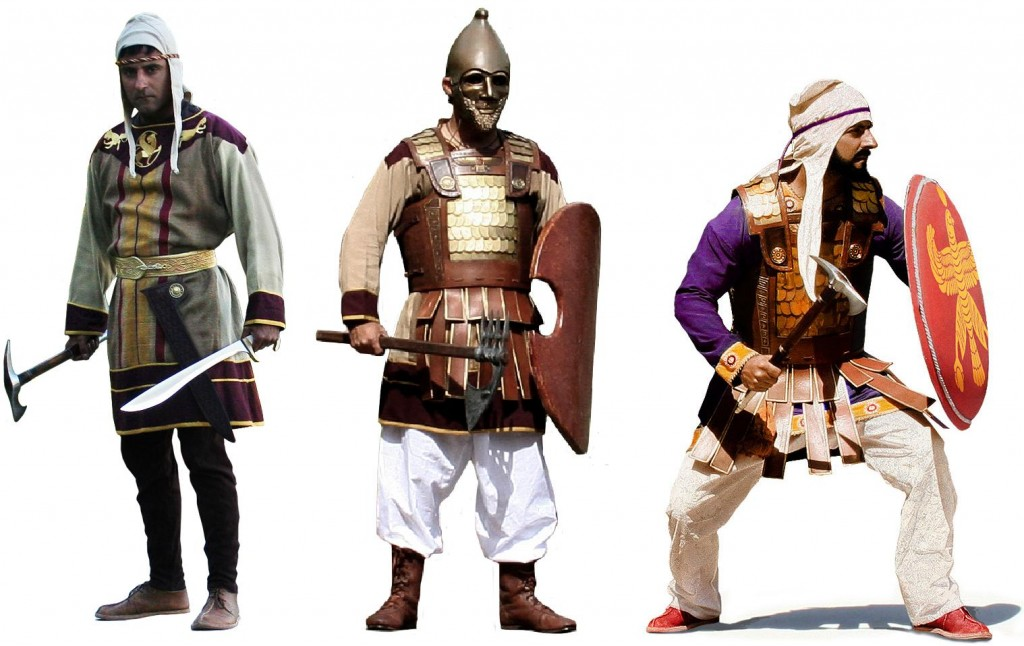
\includegraphics[width=\linewidth]{ModernImmortalReco.jpg}
  \captionsetup{justification=raggedleft}
  \caption{\ul{Modern Reconstruction of Immortals}}
  \sourceR{\cite{farrokh_2013}}
  \label{img:ImmortalModern}
\end{wrapfigure}

\par\vspace{1em}

In 512 BC, the Ionian states began a revolt against the Persians, who had
begun to enact enormous taxes on their satraps, the Ionians having joined the
empire in order to avoid a Spartan invasion years prior.\footnotemark
Athens joined the expedition in 499 BC, sending part of a fleet to sack the Persian
satrapy of Sardis. The houses, however, were made of reed, and as one soldier
set a building on fire, the entire city burned to the ground.\footnotemark[\value{footnote}]
\footnotetext{\cite[19-21]{green_darius_west}}

\par\vspace{1em}

Darius, the King of Persia, naturally was furious at the loss of Sardis,
Herodotus claims he cursed vengeance on Athens and the Ionians.
\footcite[Book 5.105]{herodotus_1920}
The Ionian revolt didn't last long, with Ionian cities quickly falling to the
Persian armies before a reasonable force landed at Marathon.
\footnotemark
The Athenians marched to Marathon to oppose the Persian army
at the behest of Miltiades, who argued that a siege could put Athens at risk of
treachery from inside. At Marathon, the armies faced off in their
respective camps for three days, neither making a move. The Athenians didn't
want to take on the Persians on the open plain, as the Persians had cavalry,
archers and a numerical advantage.\footnotemark[\value{footnote}]
They also probably hoped for the Spartan force to arrive, who famously claimed
to not wish to march until the full moon.
\footnotetext{\cite[30, 32]{green_darius_west}}\footcite[Book 6.106]{herodotus_1920}

\par\vspace{1em}

Attempting to slip the cavalry away and attack Athens with the help of some
Attic traitors, a scout serving in the Persian camp warned Miltiades, the Greek
commander of the lack of cavalry.
\footcite[35]{green_darius_west}
The Persians had set up their defensive line
no more than a mile from the Greeks, and Militades sensed a victorious moment
coming. He ordered a charge `at full run' at the Persian lines,\footcite[Book 6.112]{herodotus_1920}
hoping to dodge the Persian arrow-fire.
The Greeks used much longer spears than the Persians, who didn't even have their
immortal unit with them at the time, so there was little issue keeping the
Persian infantry at bay once the lines were engaged, and they had nothing to
fear from arrows or cavalry. Also, they were men fighting for their freedom,
not conscripted soldiers. The Greeks had no issues creating a route on the wings,
and disengaged from here to tackle the more experienced troops who had broken
through the lines in the centre. The Persians lost 6,400 men in this battle,
\footcite[37]{green_darius_west} and
Athens could finally claim a military victory against the greatest force on Earth.


\par\vspace{1em}

A nation resisting Persian subjugation could never stand for long without
becoming the Emperor's target once again, and the Greek states were no
exception. Darius' successor Xerxes would attempt to sack Greece for its worth
and prove that Persia had military dominance in all her Empire. So once again, in 480 BC,
the Persian's sailed for Greece, landing just North of Thessaly. The Thessalonians
had promised Persia full support for the invasion, \footcite[52]{green_legacy_marathon}
though Morris and Powell argue that the site was unsuitable for defence
as there was a second entry to the town, allowing the army to be easily
flanked. \footcite[260]{morris_powell_2010} Either way, the armies the Greeks
mustered, with Sparta finally willing to join to defend the nation, set up
a defensive line at \emph{Thermopylae}. The Greeks knew they
couldn't take on the Persian armies on the open plain, they were far outnumbered.
Herodotus put the Persian army size at five million men,
\footcite[Book 7.185-6]{herodotus_1920}
though in reality it was probably between eighty thousand \footcite{kim_grecopersia_2017}
and five hundred thousand, \footcite[285]{morris_powell_2010} more than
enough men to take on Greece.

\par\vspace{1em}

Thermopylae was an ideal location for a defensive stand. The narrow passage
between the mountains and the sea meant that only a small force could be engaged
at any one time, removing numerical advantages and flanking
as an option, so in theory the Greeks could hold the pass
so long as they had men still breathing. The Greeks also had the advantage
of longer spears, and well trained men. \footcite[135]{green_corner_freedom}
Despite having the Immortals present
at the battle, who supposedly were superior fighters to even the Spartans,
\footcite{kim_grecopersia_2017}
their shorter spears meant that they couldn't inflict damage on the hoplites.
The Persian arrow fire also didn't seem to concern the Spartans, one of
whom joked `if the Medes darken the sun, we shall have our fight in the shade.'
\footcite[Book 7.226]{herodotus_1920}
Despite a relentless Persian onslaught, the Greeks held all the advantages,
even pulling off a successful feigned retreat, a dangerous but effective move.
Eventually, a pro-Persian traitor, Ephialtes, showed the Persian army a way behind the pass,
allowing the stalemate to become a slaughter. King Leonidas of Sparta, so the
legend says, dismissed the Peloponnesian troops after learning of the treachery,
trying to avoid mass slaughter, and remained with only three hundred Spartiate,
that is, Spartan citizens and warriors, for the final battle.
All three hundred Spartans were killed, including Leonidas,
unable to fight on two fronts. \footcite[139-42]{green_corner_freedom}

\par\vspace{1em}

The other great land battle of the
Greco-Persian Wars was Plataea. The Greek Allies attempted one last stand after
the sack of Athens, forming up across the plain from the Persians, on the
high ground at Plataea. Outnumbered between two or three to one,
\footcite[Book 9.31-2]{herodotus_1920}
the Allies needed every advantage available, and the high ground ensured a
direct charge would be too costly, and it proved to be. The Persian commander
Mardonius started cavalry hit-and-run tactics to try and lure the Greeks down the
hill, but an Athenian archer band was able to kill the cavalry commander,
forcing retreat.\footnotemark
The Greeks were able to form up a better defensive
position, though the details of which are fiercely disputed.\footnotemark[\value{footnote}]
\footnotetext{\cite[246-7]{green_last_enemy}}
Mardonius was beginning to become frustrated after several days of inaction,
and despite the warnings of his soothsayers,
started attacking the Greek supply lines. \footcite[\emph{Arist.}15]{plutarch_1920}
The Greeks were forced to withdraw to the front of the Plataean City, a couple of
regiments at a time, wherein the Persians began an all-out assault. The Spartans
tried their false retreat again, but instantly called for help from the withdrawing
Athenians, who complied instantly. \footnotemark
Against all odds, the Greeks began to win the battle, with the Persians out
of position.
Pausanias, the Greek commander, ordered them to `take no prisoners,' and only
called off the bloodthirsty men when but three thousand Persians still
breathed.\footnotemark[\value{footnote}]
\footnotetext{\cite[265, 270]{green_last_enemy}}
This marked the final appearance of Persia in the Greek mainland in the
fifth century BC.
\par\vspace{1em}

Overall Greece should have had no chance against the Persians, being overall
undertrained and outnumbered for most of the war. However a combination
of bad luck and bad commanding, as well as superior equipment and a cause
for which to fight gave the Greeks victory in unlikely circumstances.

% Bib page
\newpage

\listoffigures
\printbibliography


\end{document}
